Nesta parte, consideraremos um cenário com \textit{imperfect compliance}\footnote{Imperfect compliance ocorre em experimentos, como RCTs, quando os indivíduos não seguem perfeitamente as alocações designadas, resultando em situações em que alguns no grupo de tratamento não recebem o tratamento, e outros no grupo de controle acabam recebendo-o. Isso compromete a adesão completa ao design experimental e pode introduzir viés nas estimativas causais. Para lidar com esse problema, utilizam-se métodos como o Intention-to-Treat (ITT), que mede o efeito com base nas alocações originais, independentemente da adesão, refletindo o impacto de oferecer o tratamento; e o Local Average Treatment Effect (LATE), que isola o efeito causal sobre os compliers (indivíduos que seguem as alocações designadas), geralmente estimado com variáveis instrumentais. Essas abordagens permitem obter inferências robustas mesmo diante de conformidade imperfeita, comum em experimentos aplicados.}, isto é, quando alguns indivíduos não seguem a designação de tratamento. Agora, $Z_i = 1$ se refere a receber uma vaga numa escola de ensino técnico, enquanto que $Z_i = 0$ se refere a não ter recebido. Ainda, $D_i = 1$ se refere ao aluno ter se matriculado na escola de ensino técnico e $D_i = 0$ significa que o aluno não se matriculou nessa escola.  No nosso caso, \textit{imperfect compliance} significa que alguns alunos que receberam uma vaga aleatoriamente, não se matricularam ($Z_i =1$, mas $D_i = 0$), enquanto que outros alunos que não receberam uma vaga de forma aleatória acabaram se matriculando ($Z_i = 0$, mas $D_i = 1$).

Neste caso, se utilizarmos a oferta de vaga numa escola de ensino técnico, $Z_i$, como variável de tratamento, estaríamos identificando o Intention-to-Treat (ITT). Esse parâmetro de interesse captura o efeito de oferecer o tratamento, independente da adesão. Para calcularmos o MDE do ITT, utilizamos a mesma fórmula dada em \ref{mde2}. No entanto, em casos de \textit{imperfect compliance}, estaremos muitas vezes interessados no Local Average Treatment Effect (LATE) é dado por $\beta^{\text{LATE}} = \mathbb{E}[Y_i(1) - Y_i(0) \mid C]$, onde $C$ é o grupo de \textit{compliers}, isto é, quando $Z_i = D_i$. Ele pode ser identificado por

    $$
    \beta^{\text{LATE}} = \frac{\mathbb{E}[Y_i \mid Z_i = 1] - \mathbb{E}[Y_i \mid Z_i = 0]}{\mathbb{E}[D_i \mid Z_i = 1] - \mathbb{E}[D_i \mid Z_i = 0]}
    $$
Podemos estimar $\beta^{\text{LATE}}$ pela divisão da diferença de médias de $Y_i$ entre o grupo de tratamento e controle, $\Bar{Y}_1 - \Bar{Y}_0$, pela diferença de médias de $D_i$ entre o grupo de tratamento e controle, $\Bar{D}_1 - \Bar{D}_0$, a qual chamaremos de \textit{take up} diferencial. No nosso exemplo prático, o denominador do estimador do LATE, $\Bar{D}_1 - \Bar{D}_0$, pode ser interpretado como a diferença de matrícula na escola de ensino técnico entre os alunos do grupo de tratamento e controle. Para calcularmos o MDE do estimador do LATE, basta dividirmos a fórmula dada em \ref{mde2} por essa diferença de adesão ao tratamento:

\begin{equation}\label{mdeiv}
    MDE = (t_{\frac{\alpha}{2}} + t_{1-\kappa})\sqrt{\frac{1}{p(1-p)}\frac{\sigma^2}{N}}\frac{1}{(\Bar{D}_1 - \Bar{D}_0)}
\end{equation}
  

Pelo fato de existir \textit{imperfect compliance}, o MDE pode ser muito maior do que no caso de \textit{perfect compliance}, visto na subseção anterior. Por exemplo, se apenas metade dos alunos do grupo de tratamento se matricularem nas escolas e nenhum aluno do grupo de controle se matricular, teremos que $\Bar{D}_1 - \Bar{D}_0 = 50\%$, logo, nesse experimento seria necessário uma amostra 4 vezes maior para ter o mesmo MDE de um experimento com 100\% de compliance. Uma vez que o MDE é linear na proporção de compliance, mas só aumenta numa razão de raiz quadrada com o tamanho de amostra N.

\subsection{\sc Praticando: Fórmula Analítica}

Agora, iremos calcular o MDE através da fórmula analítica para o caso de \textit{imperfect compliance}. Assim como na seção anterior, começaremos o código limpando o ambiente e carregando o pacote \texttt{tidyverse}. Em seguida, definiremos os parâmetros que ficaram fixos no cálculo do MDE.

\begin{boxH}
\begin{lstlisting}[language = R]
# Limpar o ambiente 
rm(list=ls())

# Carregando pacotes necessários
library(tidyverse)

# Parâmetros para cálculo analítico do MDE
t.kappa = 0.84 # poder de 80%
t.alpha = 1.96 # nível de significância de 5%
P = 0.5 # Porcentagem de tratados de 50%
\end{lstlisting}
\end{boxH}

Note que não definimos o tamanho do parâmetro de \textit{take up} diferencial. Isso porquê iremos criar a função do cálculo do MDE em termos tanto do tamanho da amostra, quanto do \textit{take up} diferencial. No bloco de código abaixo, a função \texttt{MDE.IV} se refere à equação \eqref{mdeiv}, em que o argumento \texttt{N} se refere ao tamanho da amostra, $N$, e o argumento \texttt{take.up} se refere ao \textit{take up} diferencial, $\Bar{D}_1 - \Bar{D}_0$.

\begin{boxH}
\begin{lstlisting}[language = R]
# Fórmula analítica do MDE em função de N e da % de take up

MDE.IV = function(N,take.up){(t.kappa+t.alpha)*((1/(P*(1-P)))^0.5)*((1/N)^0.5*(1/take.up))}


\end{lstlisting}
\end{boxH}

No bloco de código abaixo, fazemos o gráfico da Figura \ref{fig:mdeiv}. Nele, temos o MDE em termos de desvio padrão no eixo Y e o tamanho da amostra variando de 500 até 3500 no eixo X. Além disso, criamos três curvas, uma para cada valor de \textit{take up} diferencial: 50\%, 60\% e 70\%. Note que quanto menor o \textit{take up} diferencial, maior o valor do MDE. 

\begin{boxH}
\begin{lstlisting}[language = R]
# Gráfico do MDE variando N, para take up de 50%, 60% e 70%

ggplot() + xlim(500, 3500) +
  geom_function(fun = MDE.IV, args = list(take.up = 0.50), aes(colour = "Take Up = 50%"), linewidth = 0.8) +
  geom_function(fun = MDE.IV, args = list(take.up = 0.60), aes(colour = "Take Up = 60%"), linewidth = 0.8) +
  geom_function(fun = MDE.IV, args = list(take.up = 0.70), aes(colour = "Take Up = 70%"), linewidth = 0.8) +
  labs(y = "MDE", x = "N") +
  theme_classic() +
  guides(colour=guide_legend(title="Take Up"))

\end{lstlisting}
\end{boxH}

\begin{figure}[h]
    \centering
    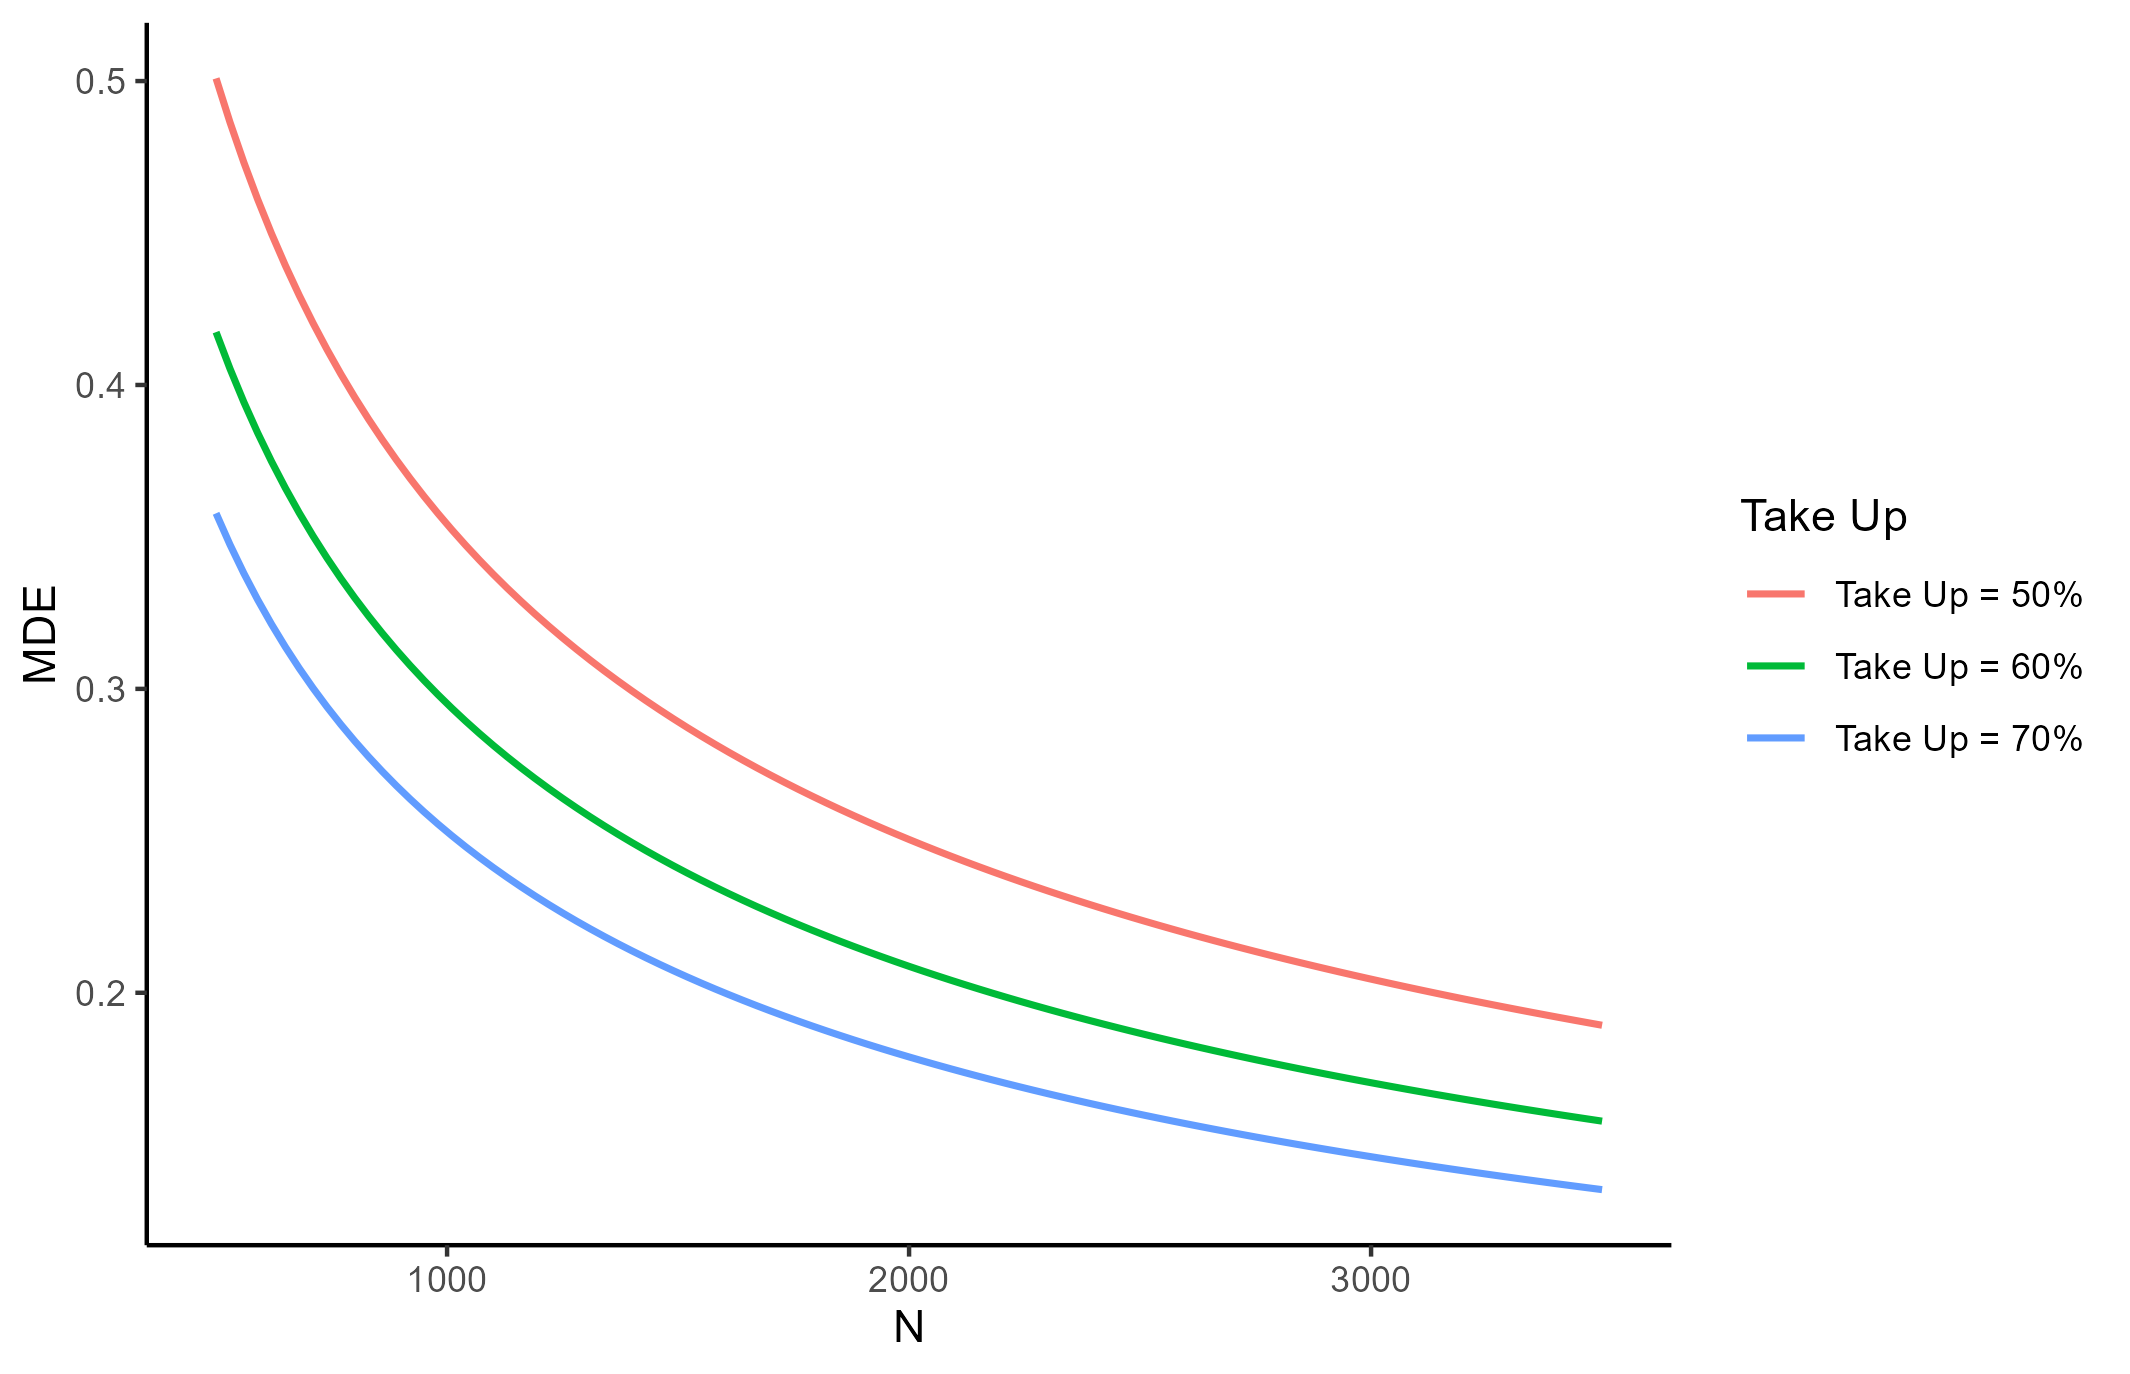
\includegraphics[width=\linewidth]{Figuras/mde_iv.png}
    \caption{Gráfico do MDE em termos de desvio padrão variando o tamanho da amostra de 500 a 3500 para diferentes tamanhos de \textit{take up}.}
    \label{fig:mdeiv}
\end{figure}

\subsection{\sc Praticando: Simulações}

Agora iremos calcular o MDE para o caso de \textit{imperfect compliance} a partir de simulações. Primeiramente, iremos limpar o ambiente e carregar os pacotes necessários. Desta vez, iremos utilizar também o pacote \texttt{ivreg}, que nos permitirá fazer regressões de 2SLS.\footnote{Uma regressão de MQO em dois estágios (Two-Stage Least Squares – 2SLS) é uma técnica usada quando há um problema de endogeneidade em um modelo de regressão. O 2SLS funciona como se estivéssemos ``filtrando'' as partes problemáticas do tratamento (estar matriculado numa escola de ensino técnico), usando uma variável auxiliar (ter recebido a oferta de um sorteio aleatório) para isolar o efeito puro da variável que realmente nos interessa.} Ainda, iremos escolher uma \textit{seed} aleatória. Novamente, escolhemos a \textit{seed} 42. Por fim, carregamos novamente a base de dados \texttt{base\_rct.csv}.

\begin{boxH}
\begin{lstlisting}[language = R]
# Limpar o ambiente 
rm(list=ls())

# Carregando pacotes necessários

library(tidyverse)
library(randomizr)
library(ivreg)

# Fazendo com que as simulações se tornem reproduzíveis
set.seed(42)

# Base de dados
base_rct <- read.csv("Base/base_rct.csv")
\end{lstlisting}
\end{boxH}

O processo para estimarmos o erro padrão do estimador de 2SLS é semelhante ao caso do MQO na seção anterior. No entanto, agora iremos aleatorizar o instrumento $Z_i$. Para determinarmos o tratamento, $D_i$, criaremos uma variável auxiliar, \texttt{aux}. Ela assumirá uma distribuição uniforme [0,1] e a variável de tratamento dependerá dos valores do instrumento e da variável auxiliar. Essa variável determinará a probabilidade com que o aluno irá de fato se matricular numa escola de ensino técnico. No exemplo de código abaixo, caso o aluno não receba o incentivo da vaga na escola de ensino técnico ($Z_i = 0$), a probabilidade dele se matricular na escola é de 20\%, enquanto que, caso o aluno receba o incentivo ($Z_i = 1$), a probabilidade dele se matricular é de 75\%. Portanto, o \textit{take up} para cada iteração da simulação será aproximadamente de 75\% - 20\% = 55\%. 

O restante da simulação é análogo ao caso com \textit{perfect compliance}: \textit{(i)} rodamos a regressão de 2SLS para cada iteração; \textit{(ii)} armazenamos o erro padrão do estimador de 2SLS num vetor e \textit{(iii)} calculamos o MDE utilizando a média dos erros padrão estimados. 

\begin{boxH}
\begin{lstlisting}[language = R]
# Criando vetor com 100 entradas para armazenar os erros padrões
se_late <- c(rep(NA, 100))

# Simulando 100 vezes o erro padrão
for (i in 1:100) {
  
  Z <- simple_ra(N = nrow(base_rct), prob = 0.5) # Aleatorizando o instrumento
  df <- cbind(base_rct, Z) # juntando bases
  
  df <- df %>% # criando variável auxiliar para criar variável de tratamento
    mutate(aux = runif(nrow(base_rct))) %>%
    mutate(D = case_when(Z==0 & aux<0.2 ~ 1,
                         Z==0 & aux>0.2 ~ 0,
                         Z==1 & aux<0.75 ~ 1,
                         Z==1 & aux>0.75 ~ 0)) %>%
    select(-aux)
  
  reg_late <- ivreg(y ~ D|Z, data = df) # regressão 2sls
  se_late[i] <- summary(reg_late)$coefficients[2,2] # armazenando erro padrão
  
}

# Calculando MDE
MDE_late = 2.8*mean(se_late)
print(MDE_late)
\end{lstlisting}
\end{boxH}